\chapter{de-Sitter-Horizonte und kosmologische Wahrscheinlichkeit}

\lectureoverview{Ein Horizont ist nicht bloß eine Kausalgrenze. Für einen stationären Beobachter ist er ein thermisches System: Ein Thermometer im Eigenabstand \(\rho\) vom Horizont zeigt eine Temperatur in der Größenordnung von \(1/(2\pi\rho)\) an, während die gravitative Rotverschiebung die Strahlung, die in großer Entfernung gemessen wird, deutlich abkühlt. Wir übertragen die Erkenntnisse über Schwarze Löcher auf den de-Sitter-Raum, leiten den festen Horizontsradius \(H^{-1}\) her und geben die Metrik des statischen Beobachtergebiets an. In der zweiten Hälfte der Vorlesung führen die thermodynamischen Überlegungen zu beunruhigenden Konsequenzen: endliche de-Sitter-Entropie, Poincaré-Wiederkehr, Boltzmann-Gehirne, ewige Inflation und das Maßproblem. Eine abschließende Diskussion unterscheidet die exakten supersymmetrischen Strukturen der Stringtheorie von dem noch unbekannten Rahmen, der unsere Welt beschreiben könnte.}

\section{Was es bedeutet, dass ein Horizont heiß ist}

Wir beginnen vor der eigentlichen Vorlesung mit der Frage, die die Richtung des Abends bestimmt.

\begin{classroomqa}
\audiencequestion{Ein kosmischer Horizont enthält kein Schwarzes Loch. Durch welchen Mechanismus kann er dennoch heiß sein?\lecturetimestamp{00:00:17}}
\lecturerresponse{Der Mechanismus ist derselbe wie bei einem Horizont eines Schwarzen Lochs. Die entscheidende Frage ist operational: Was zeigt ein Thermometer an, das nahe am Horizont gehalten wird, und welche Strahlung erreicht einen weit entfernten Beobachter?}
\end{classroomqa}

Das erste Experiment ist lokal. Man hält ein Thermometer im festen Eigenabstand \(\rho\) von einem beliebigen glatten, nichtentarteten Horizont. Nahe genug am Horizont hat die Geometrie die universelle Rindler-Form, und das Thermometer zeigt
\begin{equation}
T_{\rm local}(\rho)\simeq \frac{1}{2\pi\rho}
\label{eq:l09-local-temperature}
\end{equation}
in Einheiten mit \(\hbar=c=k_B=1\) an. Mit wieder eingesetzten Konstanten ergibt sich
\begin{equation}
k_B T_{\rm local}(\rho)\simeq \frac{\hbar c}{2\pi\rho}.
\end{equation}
Die Divergenz für \(\rho\to0\) bedeutet nicht, dass ein hineinfallender Beobachter auf einen gewöhnlichen materiellen Brennofen trifft. Es handelt sich um die Temperatur, die ein Beobachter misst, der knapp außerhalb des Horizonts stationär bleibt und deshalb immer stärker beschleunigen muss.

Das einleitende Gespräch unterscheidet außerdem drei leicht zu verwechselnde Begriffe: Energie, Temperatur und Entropie.

\begin{classroomqa}
\audiencequestion{Wenn Photonen in ein Schwarzes Loch geschickt werden, messen wir dann weiterhin dieselbe Entropie, oder ändert sich nur die Energie?\lecturetimestamp{00:01:22}}
\lecturerresponse{Sobald ein Photon hinter dem Horizont unzugänglich wird, ist zusätzliche Information verborgen. In der hier verwendeten vereinfachten Sprache von Bits kann ein Photon ein zusätzliches Bit verbergen und so die Entropie erhöhen. Energie, Temperatur und Entropie hängen zusammen, sind aber nicht austauschbar.}
\end{classroomqa}

\editorialnote{Bei einem physikalischen Schwarzen Loch ist die Entropieänderung thermodynamisch durch \(dS=dE/T_H\) festgelegt; sie beträgt nicht unabhängig von der Energie für jedes Photon ein Bit. Die Aussage über ein Bit ist die informationstheoretische Idealisierung der Vorlesung.}

Die Umgebung des Horizonts emittiert und absorbiert fortwährend hochfrequente Quantenfluktuationen. Für den stationären Beobachter erscheinen diese Fluktuationen durch den Horizont thermisch. Das wirft jedoch unmittelbar eine Frage auf: Wenn die Umgebung beliebig heiß ist, warum wird ein weit entfernter Beobachter dann nicht von Photonen beliebig hoher Energie geblendet?

\section{Rotverschiebung und Hawking-Temperatur}

Eine gewöhnliche heiße Wand bleibt eine Quelle hochfrequenter Strahlung, auch wenn wir weit von ihr entfernt stehen. Bei einem Horizont ist es anders, denn seine Strahlung muss eine gravitative Rotverschiebung durchlaufen. Die Geschwindigkeit des Photons bleibt \(c\); was abnimmt, ist seine Energie:
\begin{equation}
E=\hbar\omega,
\qquad
\omega_{\rm received}<\omega_{\rm emitted}.
\end{equation}
Die im Vortrag verwendete Analogie mit einem Stück Kreide hilft nur bis zu diesem Punkt. Ein geworfener Stein wird beim Aufsteigen langsamer, während ein Photon sich weiterhin mit Lichtgeschwindigkeit bewegt, obwohl seine Frequenz und Energie abnehmen.

Für ein Schwarzschild-Schwarzes-Loch beträgt die Temperatur, die ein Beobachter im Unendlichen misst,
\begin{equation}
T_H=\frac{1}{8\pi M}
\label{eq:l09-hawking-natural}
\end{equation}
in Einheiten mit \(G_N=\hbar=c=k_B=1\). In gewöhnlichen Einheiten gilt
\begin{equation}
T_H=\frac{\hbar c^3}{8\pi G_N M k_B}.
\label{eq:l09-hawking-full}
\end{equation}

\begin{figure}[htbp]
\centering
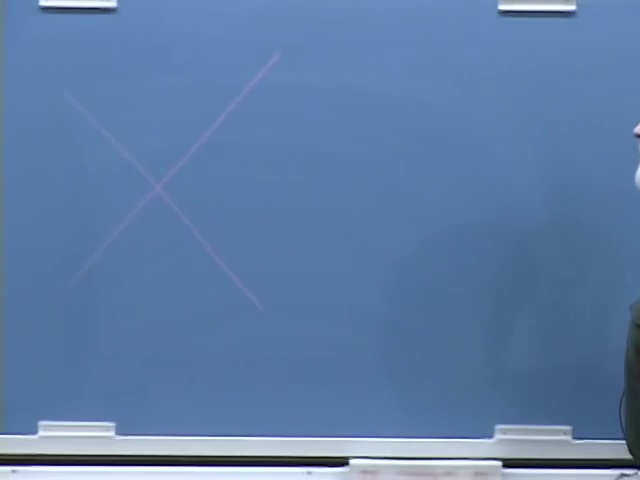
\includegraphics[width=0.68\textwidth]{lecture_09_figure_02.png}
\caption{Die Hawking-Temperatur \(T_H=1/(8\pi M)\) in natürlichen Einheiten.}
\lectureframe{00:08:12}
\end{figure}

Ein größeres Schwarzes Loch ist kälter. Die Vorlesung erklärt dies, indem sie ein typisches Photon rückwärts verfolgt. Thermische Photonen haben eine charakteristische Energie \(E_\gamma\sim T_H\). Ein Photon, das das Unendliche mit einer Energie in der Größenordnung von \(M^{-1}\) erreicht, hatte nahe am Horizont eine viel größere lokale Energie. Bei einem größeren Schwarzen Loch ist die Rotverschiebung zwischen der Schicht nahe dem Horizont und dem Unendlichen stärker; dadurch ist die asymptotische Temperatur niedriger.

\begin{classroomqa}
\audiencequestion{Wenn die Schwarzschild-Zeit am Horizont einfriert, sollten wir dann das Photon verfolgen, das ursprünglich hineingefallen ist und das Schwarze Loch aufgebaut hat?\lecturetimestamp{00:04:19}}
\lecturerresponse{Für die Temperaturfrage verfolgen wir die nach außen emittierten Photonen. Sie beginnen mit sehr hoher lokaler Frequenz, verlieren beim Aufsteigen Energie und treffen als Hawking-Strahlung ein. Was mit dem ursprünglich hineingefallenen Photon geschieht, ist eine gesonderte Frage der Information.}
\end{classroomqa}

\section{Die Planck-Schicht und der gestreckte Horizont}

Wie nahe am Horizont gilt die lokale Beziehung in Gleichung~\eqref{eq:l09-local-temperature}? Die Vorlesung setzt die Planck-Länge als den kleinsten sinnvollen Abstand in der semiklassischen Beschreibung an. Das legt eine dünne Schicht nahe, ungefähr eine Planck-Länge außerhalb des mathematischen Horizonts, die von Fluktuationen auf der Planck-Skala erfüllt ist. Sie emittiert und absorbiert fortwährend.

Die meisten emittierten Quanten entkommen nicht. Nur diejenigen, die in einen sehr schmalen Kegel nach außen gerichtet sind, entgehen dem Zurückfallen. Quanten, die unter allgemeinen Winkeln ausgesandt werden, kehren zum Horizont zurück. Auslaufende und einlaufende Anregungen stoßen zusammen und erzeugen Paare und andere Teilchen; in diesem Sinne enthält die stationäre Beschreibung eine dünne Schale extrem heißer Materie.

\begin{figure}[htbp]
\centering
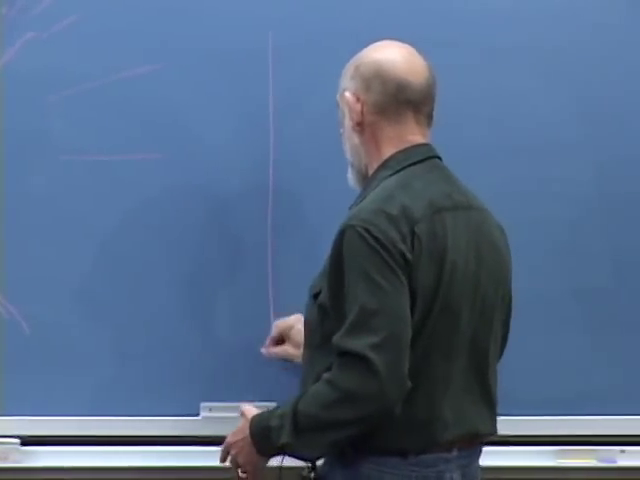
\includegraphics[width=0.74\textwidth]{lecture_09_figure_03.png}
\caption{Der schmale Entweichungskegel für Strahlung nahe dem Horizont. Die meisten lokal emittierten Quanten kehren zum Horizont zurück.}
\lectureframe{00:11:38}
\end{figure}

Es gibt ein ergänzendes raumzeitliches Bild. Weit entfernt von einem Horizont lässt sich eine virtuelle Fluktuation schematisch als kurze geschlossene Schleife darstellen: Eine Teilchen-Antiteilchen-Anregung entsteht und verschwindet, bevor sie zu einem asymptotischen Zustand werden kann. Nahe einem Horizont kann eine Fluktuation die Kausalgrenze übergreifen. Für den äußeren Beobachter sieht der außerhalb liegende Teil wie ein vom Horizont emittiertes und später wieder absorbiertes Teilchen aus. Ein sehr kleiner Anteil entkommt und wird zu Hawking-Strahlung.

\begin{classroomqa}
\audiencequestion{Erstreckt sich eine solche Fluktuation im Außengebietsdiagramm von \(t=-\infty\) bis \(t=+\infty\)?\lecturetimestamp{00:15:00}}
\lecturerresponse{Der exakte klassische Horizont führt zu dieser singulär anmutenden Beschreibung. In der Praxis ersetzen wir ihn durch einen gestreckten Horizont, eine zeitartige Fläche etwa eine Planck-Länge außerhalb. Emission und Reabsorption finden dann zu endlichen äußeren Zeiten statt.}
\end{classroomqa}

\begin{figure}[htbp]
\centering
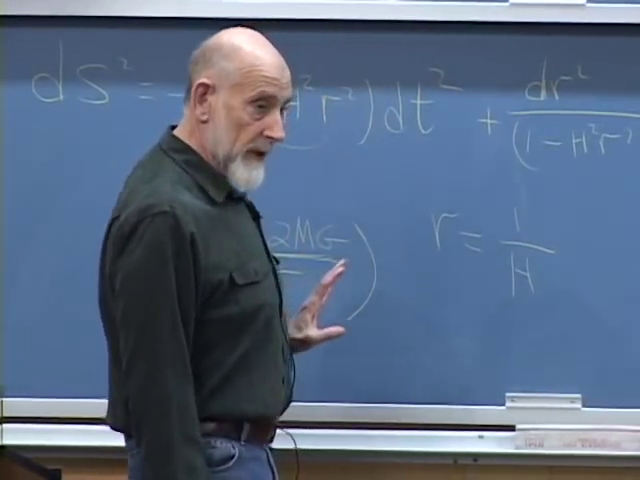
\includegraphics[width=0.72\textwidth]{lecture_09_figure_04.png}
\caption{Der klassische Horizont und der nahe gelegene gestreckte Horizont, der in der Beschreibung des Außengebiets verwendet wird.}
\lectureframe{00:15:52}
\end{figure}

Der gestreckte Horizont ist keine neue invariante Grenze. Er ist eine effektive Fläche an der Stelle, an der die semiklassische Geometrie ihre Zuverlässigkeit verliert. Quantenfluktuationen der Materie und der Geometrie selbst verwischen die genaue Lage auf Planck-Skalen. Diese Konstruktion fasst jene Unschärfe in einer Fläche zusammen, auf der die Beschreibung des Außengebiets endlich bleibt.

Nichts in dieser lokalen Argumentation verrät, ob der Horizont zu einem Schwarzen Loch oder zu einem beschleunigt expandierenden Universum gehört. Das ist die Brücke zum de-Sitter-Raum.

\section{Der de-Sitter-Raum in expandierenden Koordinaten}

Die formale Vorlesung beginnt mit der räumlich flachen Schichtung der de-Sitter-Raumzeit:
\begin{equation}
ds^2=-dt^2+e^{2Ht}d\mathbf{x}^2,
\qquad
d\mathbf{x}^2=dx^2+dy^2+dz^2.
\label{eq:l09-flat-slicing}
\end{equation}
Die Konstante \(H\) ist die Expansionsrate des de-Sitter-Raums. Der Faktor tritt als \(e^{2Ht}\) auf, weil die Metrik das Abstandsquadrat misst; ein festes Koordinatenintervall hat die physikalische Länge
\begin{equation}
D(t)=e^{Ht}\lvert\Delta\mathbf{x}\rvert.
\end{equation}

\begin{figure}[htbp]
\centering
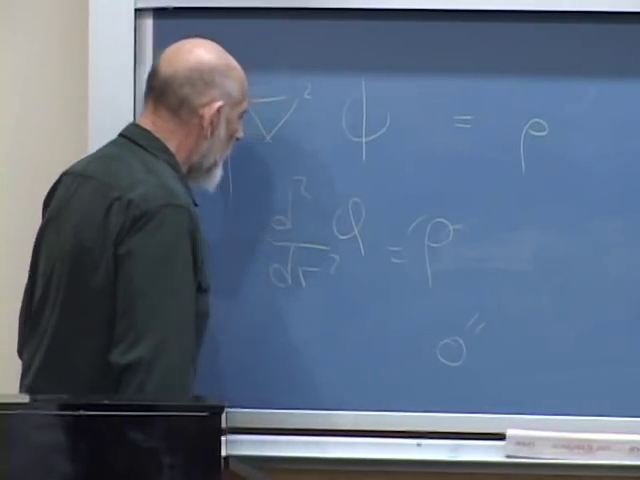
\includegraphics[width=0.78\textwidth]{lecture_09_figure_05.png}
\caption{Die exponentiell expandierende de-Sitter-Metrik in flachen Koordinaten.}
\lectureframe{00:18:50}
\end{figure}

Diese Koordinaten machen die Expansion anschaulich, legen aber die zukünftige Unendlichkeit unendlich weit oben auf der Seite. Um sie auf die Tafel zu holen, führen wir die konforme Zeit ein:
\begin{equation}
\eta=-\frac{1}{H}e^{-Ht},
\qquad
-\infty<\eta<0.
\label{eq:l09-conformal-time}
\end{equation}
Dann gilt
\begin{equation}
dt=\frac{d\eta}{-H\eta},
\qquad
e^{Ht}=-\frac{1}{H\eta},
\end{equation}
und Gleichung~\eqref{eq:l09-flat-slicing} wird zu
\begin{equation}
ds^2=\frac{1}{H^2\eta^2}
\left(-d\eta^2+d\mathbf{x}^2\right).
\label{eq:l09-conformal-metric}
\end{equation}
Für \(t\to+\infty\) gilt \(\eta\to0^{-}\). Die unendliche Eigenzeit wird auf die endliche horizontale Linie \(\eta=0\) abgebildet.

\editorialnote{Die Zeittransformation wird beim Anschreiben an der Tafel mehrfach korrigiert. Gleichung~\eqref{eq:l09-conformal-time} ist die konsistente Form: Frühe kosmische Zeiten entsprechen \(\eta\to-\infty\), und die zukünftige Unendlichkeit entspricht \(\eta\to0^{-}\).}

\begin{figure}[htbp]
\centering
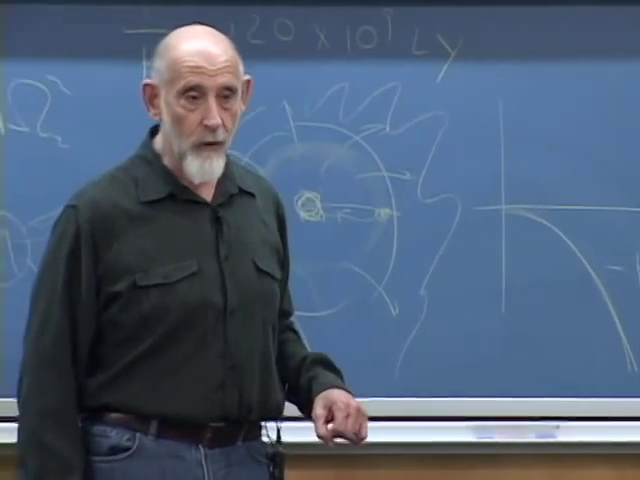
\includegraphics[width=0.82\textwidth]{lecture_09_figure_06.png}
\caption{Die Transformation zur konformen Zeit und die konform flache Metrik.}
\lectureframe{00:21:24}
\end{figure}

Der konforme Faktor multipliziert sowohl den Zeit- als auch den Raumterm und verändert daher die Nullrichtungen nicht. Für einen radialen Lichtstrahl gilt
\begin{equation}
ds^2=0
\quad\Longrightarrow\quad
-d\eta^2+dx^2=0
\quad\Longrightarrow\quad
\frac{dx}{d\eta}=\pm1.
\label{eq:l09-null-rays}
\end{equation}
Im konformen Diagramm bewegt sich Licht daher unter \(45^\circ\). Deshalb ist diese Koordinatentransformation nützlich: Die kausale Erreichbarkeit wird sichtbar.

\section{Der Kausalbereich eines einzelnen Beobachters}

Man stelle sich einen Beobachter vor, dessen Weltlinie unendlich lange fortbesteht. Im kompakten Diagramm endet sie in einem Punkt auf \(\eta=0\). Jedes Signal, das der Beobachter jemals empfangen kann, liegt innerhalb des rückwärts gerichteten Lichtkegels dieses Endpunkts. Ereignisse außerhalb des Kegels können mit dem Beobachter niemals in Verbindung treten, wie lange er auch wartet.

\begin{figure}[htbp]
\centering
\includegraphics[width=0.78\textwidth]{lecture_09_figure_07.png}
\caption{Der rückwärts gerichtete Grenzlichtkegel eines Beobachters in konformen de-Sitter-Koordinaten.}
\lectureframe{00:24:38}
\end{figure}

Ein zweiter Beobachter hat einen anderen Kegel. Die beiden zugänglichen Gebiete überlappen sich, aber keines von ihnen umfasst die gesamte Raumzeit. Für den Rest der Argumentation nehmen wir den Standpunkt des ersten Beobachters ein und nennen diesen rückwärts gerichteten Lichtkegel den Kausalbereich des Beobachters.

Die Zeichnung scheint zu zeigen, wie der Kausalbereich in Richtung Zukunft schrumpft, doch die Koordinatenbreite ist kein Eigenabstand. Auf einer Fläche konstanter \(\eta\) beträgt das Quadrat des physikalischen Abstands zwischen dem Beobachter bei \(x=0\) und dem Horizont bei \(x=\Delta x\)
\begin{equation}
D^2=\frac{(\Delta x)^2}{H^2\eta^2}.
\label{eq:l09-horizon-distance-start}
\end{equation}
Der Horizont ist eine \(45^\circ\)-Nullgerade, die bei \(\eta=0\) endet, also gilt
\begin{equation}
\Delta x=\lvert\eta\rvert.
\end{equation}
Einsetzen ergibt
\begin{equation}
D_{\rm hor}^2=\frac{1}{H^2},
\qquad
D_{\rm hor}=\frac{1}{H}.
\label{eq:l09-horizon-radius}
\end{equation}
Der Koordinatenabstand schrumpft, aber der konforme Faktor wächst genau um den kompensierenden Betrag. Der Eigenradius des Horizonts ist konstant.

\begin{figure}[htbp]
\centering
\includegraphics[width=0.80\textwidth]{lecture_09_figure_08.png}
\caption{Die Herleitung an der Tafel, die das schrumpfende Koordinatenintervall in den festen Eigenabstand \(H^{-1}\) umwandelt.}
\lectureframe{00:28:42}
\end{figure}

\section{Das statische Beobachtergebiet}

Ein fester Horizontsradius legt Koordinaten nahe, die an den zentralen Beobachter angepasst sind. Ohne die Koordinatentransformation herzuleiten, schreibt die Vorlesung das Ergebnis an:
\begin{equation}
ds^2=
-\left(1-H^2r^2\right)d\tau^2
+\frac{dr^2}{1-H^2r^2}
+r^2d\Omega_2^2.
\label{eq:l09-static-patch}
\end{equation}
Die Koeffizienten hängen von \(r\) ab, nicht von \(\tau\). Diese Karte überdeckt das statische Beobachtergebiet,
\begin{equation}
0\le r<\frac{1}{H}.
\end{equation}

\begin{figure}[htbp]
\centering
\includegraphics[width=0.88\textwidth]{lecture_09_figure_09.png}
\caption{Die Metrik des statischen de-Sitter-Beobachtergebiets und ihr Vergleich mit dem Schwarzschild-Faktor.}
\lectureframe{00:34:22}
\end{figure}

Die Ähnlichkeit mit der Schwarzschild-Geometrie ist unmittelbar erkennbar:
\begin{equation}
f_{\rm dS}(r)=1-H^2r^2,
\qquad
f_{\rm Schw}(r)=1-\frac{2G_NM}{r}.
\end{equation}
In beiden Fällen liegt der Horizont der statischen Koordinaten dort, wo \(f(r)=0\) gilt. Für den de-Sitter-Raum gilt
\begin{equation}
1-H^2r^2=0
\quad\Longrightarrow\quad
r_H=H^{-1}.
\end{equation}
Die Karte ist dort singulär, ebenso wie die Schwarzschild-Koordinaten am Horizont eines Schwarzen Lochs singulär sind. Die globalen Geometrien unterscheiden sich dennoch in einem wichtigen Punkt. Ein Beobachter bei einem Schwarzen Loch steht außen und blickt nach innen; ein de-Sitter-Beobachter steht innen und blickt nach außen.

\begin{classroomqa}
\audiencequestion{Wie kann die Geometrie statisch sein, wenn frei gelassene Teilchen sich in einem exponentiell expandierenden Universum voneinander entfernen?\lecturetimestamp{00:36:06}}
\lecturerresponse{Statisch bedeutet nicht, dass jedes Teilchen an seinem Ort bleibt. Es bedeutet, dass die Metrikkoeffizienten und das Ergebnis eines wiederholten Experiments unabhängig vom Startzeitpunkt sind. Lässt man zwei Teilchen jetzt frei, beschleunigen sie voneinander weg; wiederholt man dasselbe Experiment später, geschieht dieselbe Bewegung.}
\end{classroomqa}

\begin{classroomqa}
\audiencequestion{Sehen die beiden auseinanderdriftenden Teilchen einander rotverschoben?\lecturetimestamp{00:38:34}}
\lecturerresponse{Ja. Ihr zunehmender Abstand führt zu einer relativen Rotverschiebung, obwohl die an den Beobachter angepasste Metrik zeitunabhängig ist.}
\end{classroomqa}

\section{Temperaturmessung von innen}

Die Strukturen nahe dem Horizont sind im Schwarzschild- und im de-Sitter-Raum lokal äquivalent. Daher emittiert und reabsorbiert auch der de-Sitter-Horizont thermische Quanten. Ein seltenes Photon bewegt sich nach innen zum zentralen Beobachter und verliert Energie, während es das Potential des statischen Beobachtergebiets hinaufsteigt. Die im Zentrum gemessene Gibbons---Hawking-Temperatur beträgt
\begin{equation}
T_{\rm dS}=\frac{H}{2\pi}
\label{eq:l09-de-sitter-temperature}
\end{equation}
in natürlichen Einheiten. Ein stationäres Thermometer bei Radius \(r\) zeigt den nach Tolman rotverschobenen Wert
\begin{equation}
T_{\rm local}(r)=
\frac{T_{\rm dS}}{\sqrt{1-H^2r^2}},
\label{eq:l09-tolman}
\end{equation}
an, der für \(r\to H^{-1}\) divergiert und nahe dem Horizont auf Gleichung~\eqref{eq:l09-local-temperature} zurückgeht.

\editorialnote{Die Vorlesung gewinnt die Größenordnung aus dem Horizontabstand und der Rotverschiebung, statt die Gleichungen~\eqref{eq:l09-de-sitter-temperature} und \eqref{eq:l09-tolman} ausdrücklich anzuschreiben. Sie geben die Standardnormierung dieser Argumentation an.}

Für die beobachtete Beschleunigung in der späten kosmischen Epoche verwendet die Vorlesung die Abschätzung für den Zeitraum
\begin{equation}
H^{-1}\sim 20\times10^9\ {\rm light\ years}.
\label{eq:l09-lecture-horizon-estimate}
\end{equation}
Ein typisches Horizontphoton hat dann eine Wellenlänge, die mit mehreren Milliarden Lichtjahren vergleichbar ist. Es handelt sich nicht um Mikrowellenhintergrundstrahlung; sie ist um vieles kälter.

Das operative Gedankenexperiment verwendet eine Angelrute im kosmologischen Maßstab. Alice bleibt bei \(r=0\), befestigt ein Thermometer an einer sehr langen Schnur, die zugleich Daten überträgt, und lässt die kosmische Abstoßung das Instrument nach außen tragen. Sie hält es knapp vor dem Horizont an, wartet auf die Rückkehr des Signals und stellt eine hohe lokale Temperatur fest. Das Thermometer neben ihr im Zentrum zeigt den kleinen Wert \(H/(2\pi)\) an. Derselbe Horizont ermöglicht beide Messwerte, weil sie bei unterschiedlichen Gravitationspotentialen gewonnen werden.

\section{Den Horizont überqueren}

Die klassische Beschreibung von außen ähnelt der bekannten Geschichte über Schwarze Löcher. Bob im Zentrum beobachtet, wie Alice sich entfernt. Ihre Signale werden zunehmend rotverschoben und treffen in immer größeren zeitlichen Abständen ein; sie scheint sich am Horizont abzuflachen und verblasst schließlich. Eine spätere Reisende, Jane, erscheint als eine weitere, dünnere Schicht in einem sedimentartigen Stapel nahe der Grenze.

\begin{classroomqa}
\audiencequestion{Überqueren Objekte aus unserer Sicht jemals den kosmischen Horizont?\lecturetimestamp{00:45:30}}
\lecturerresponse{In der klassischen Beschreibung des statischen Beobachters nicht. Ihre Signale werden rotverschoben und verblassen, während ihre scheinbare Position sich dem Horizont nähert. In ihrer eigenen frei fallenden Beschreibung überqueren sie ihn jedoch, ohne auf eine lokal singuläre Fläche zu treffen.}
\end{classroomqa}

\begin{classroomqa}
\audiencequestion{Ist der Horizont nur für Beobachter heiß, die in seiner Nähe bleiben, ohne ihn zu überqueren? Wird eine hineinfallende Beobachterin beim Durchgang nicht einfach gebraten?\lecturetimestamp{00:48:27}}
\lecturerresponse{Alice überquert ihn in ihrem eigenen Bezugssystem ungestört. Die extreme Temperatur gehört zur stationären Beschreibung. Wenn Bob darauf besteht, Alice immer näher am Horizont aufzulösen, muss er sie mit immer kürzeren Wellenlängen beleuchten. Das gedachte Heisenberg-Mikroskop deponiert dann so viel Energie, dass es das Objekt, das es beobachten soll, brät.}
\end{classroomqa}

Dies ist kein Widerspruch zwischen zwei lokalen Ereignissen. Der stationäre Beobachter und die hineinfallende Beobachterin verwenden grundverschiedene Messverfahren. Die Horizontkomplementarität fragt, wie beide Beschreibungen gültig sein können, ohne dass ein Beobachter direkt doppelte Information vergleichen kann.

\section{Ein Newtonsches Modell der Vakuumabstoßung}

An dieser Stelle fragt ein Student, was im de-Sitter-Raum an die Stelle des Gravitationspotentials eines Schwarzen Lochs tritt. Susskind entwickelt dazu ein Newtonsches Modell. Sei \(\phi\) das Gravitationspotential; dann ist die Beschleunigung eines Testteilchens
\begin{equation}
\mathbf{a}=-\boldsymbol{\nabla}\phi.
\end{equation}
Für gewöhnliche nichtrelativistische Materie lautet die Poisson-Gleichung
\begin{equation}
\nabla^2\phi=4\pi G_N\rho.
\label{eq:l09-poisson}
\end{equation}

\begin{classroomqa}
\audiencequestion{Wenn die Effekte des Schwarzen Lochs von seinem Gravitationspotential herrühren, was ist dann die entsprechende Quelle im de-Sitter-Raum?\lecturetimestamp{00:49:36}}
\lecturerresponse{Die Vakuumenergie selbst liefert eine räumlich homogene Gravitationsquelle. In einer Newtonschen Beschreibung erzeugt sie ein quadratisches Potential statt eines \(1/r\)-Potentials.}
\end{classroomqa}

\begin{figure}[htbp]
\centering
\includegraphics[width=0.78\textwidth]{lecture_09_figure_10.png}
\caption{Die Poisson-Gleichung und die schematische radiale Form mit der zweiten Ableitung aus der Vorlesung.}
\lectureframe{00:51:38}
\end{figure}

An der Tafel werden Normierung, Terme aus dem Kugelmaß, der Druck und zunächst sogar das Vorzeichen weggelassen; die Aufgabe wird so reduziert auf
\begin{equation}
\frac{d^2\phi}{dr^2}\sim H^2.
\end{equation}
Die wesentliche Folgerung ist, dass eine konstante Quelle eine quadratische Funktion ergibt. Mit dem für die Abstoßung im de-Sitter-Raum erforderlichen Vorzeichen gilt
\begin{equation}
\phi_{\rm dS}(r)=-\frac{1}{2}H^2r^2,
\qquad
a_r=-\frac{d\phi_{\rm dS}}{dr}=H^2r.
\label{eq:l09-de-sitter-potential}
\end{equation}
Die Beschleunigung zeigt nach außen und wächst linear mit dem Abstand. Die Lösung von \(\ddot r=H^2r\) lautet
\begin{equation}
r(\tau)=A e^{H\tau}+B e^{-H\tau},
\end{equation}
Der wachsende Lösungszweig ergibt somit erneut eine exponentielle Trennung.

\begin{figure}[htbp]
\centering
\includegraphics[width=0.76\textwidth]{lecture_09_figure_11.png}
\caption{Die Gleichung mit homogener Quelle und das quadratische de-Sitter-Potential.}
\lectureframe{00:53:32}
\end{figure}

\editorialnote{In der allgemeinen Relativitätstheorie hängt die Beschleunigung im Schwachfeld einer homogenen Flüssigkeit von \(\rho+3p\) ab und nicht allein von \(\rho\). Für Vakuumenergie gilt \(p=-\rho\), also ist \(\rho+3p=-2\rho\) und die Beschleunigung wirkt abstoßend. Gleichung~\eqref{eq:l09-de-sitter-potential} ist das korrekt normierte de-Sitter-Ergebnis; in der Rechnung an der Tafel werden bewusst nur der quadratische Zusammenhang und das Vorzeichen betrachtet.}

Man platziere eine gewöhnliche Masse \(M\) im Zentrum. Das qualitative Potential lautet dann
\begin{equation}
\phi(r)=-\frac{G_NM}{r}-\frac{1}{2}H^2r^2,
\label{eq:l09-combined-potential}
\end{equation}
und die radiale Beschleunigung
\begin{equation}
a_r=-\frac{G_NM}{r^2}+H^2r.
\end{equation}
Bei kleinem \(r\) überwiegt die lokale Anziehung; bei großem \(r\) die Vakuumabstoßung. Ihr Gleichgewicht liegt bei
\begin{equation}
r_\ast=\left(\frac{G_NM}{H^2}\right)^{1/3}.
\label{eq:l09-turnaround}
\end{equation}
Dies ist die saubere Fassung des Potenzialmaximums aus der Vorlesung. Sie erklärt qualitativ, warum nahe gelegene, gravitativ gebundene Systeme zusammenbleiben können, während ausreichend weit entfernte Galaxien beschleunigt auseinanderdriften.

\begin{figure}[htbp]
\centering
\includegraphics[width=0.78\textwidth]{lecture_09_figure_12.png}
\caption{Anziehung durch gewöhnliche \(1/r\)-Kraft zusammen mit dem umgekehrt gekrümmten quadratischen de-Sitter-Potential.}
\lectureframe{00:58:20}
\end{figure}

\begin{classroomqa}
\audiencequestion{Spielen gewöhnliche Kräfte weiterhin eine Rolle, oder zerreißt die Vakuumrepulsion schließlich jede Insel aus Materie?\lecturetimestamp{00:57:29}}
\lecturerresponse{Alle Kräfte müssen berücksichtigt werden. Auf hinreichend kleinen Skalen dominieren die elektromagnetische Bindung und die lokale Gravitation. Vakuumrepulsion wird erst über gewaltige Entfernungen wichtig, die durch \(H^{-1}\) und die für die gebundene Masse maßgebliche Gleichgewichtsskala bestimmt sind.}
\end{classroomqa}

\section{Eine Quelle, mehrere Bezeichnungen}

Nun hält die Diskussion inne, um die Begriffe zu klären. Vakuumenergie, kosmologische Konstante und dunkle Energie sind in dem verwendeten Modell keine drei additiven Substanzen. Sie bezeichnen ein und dieselbe Quelle mit Zustandsgleichung \(w=-1\). Man kann von einem konstanten Term in der Einsteinschen Gleichung, einer Lorentz-invarianten Energiedichte des Vakuums oder der Komponente sprechen, die die späte kosmische Beschleunigung antreibt.

\begin{classroomqa}
\audiencequestion{Treten die homogene Newtonsche Quelle und die quantenmechanische Vakuumenergie als getrennte Effekte zugleich auf?\lecturetimestamp{00:59:14}}
\lecturerresponse{Nein. Die homogene Dichte ist das Newtonsche Modell derselben Quelle. Vakuumenergie, kosmologische Konstante und in dieser Vorlesung dunkle Energie bezeichnen eine einzige physikalische Komponente.}
\end{classroomqa}

\begin{classroomqa}
\audiencequestion{Hat dasselbe Phänomen demnach sowohl eine klassische als auch eine quantenmechanische Beschreibung?\lecturetimestamp{01:00:32}}
\lecturerresponse{Sein mikroskopischer Ursprung kann quantenmechanisch sein, so wie auch ein Teil der Masse eines Elektrons einen quantenmechanischen Ursprung hat. Sobald die effektive Energiedichte bekannt ist, geht sie als gewöhnliche Quelle in die klassischen Gravitationsgleichungen ein. Den letztlichen Ursprung des beobachteten Werts kennen wir nicht.}
\end{classroomqa}

In Planck-Einheiten ist die beobachtete Vakuumenergiedichte außerordentlich klein:
\begin{equation}
\rho_\Lambda\sim10^{-123}\rho_{\rm Pl},
\label{eq:l09-planck-smallness}
\end{equation}
bis auf die verwendete Konvention für die Planck-Dichte. Diese kleine Zahl ist der Kern des Problems der kosmologischen Konstante. Sie erklärt auch, warum der Horizont so groß ist: In vier Dimensionen gilt
\begin{equation}
H^2=\frac{8\pi G_N}{3}\rho_\Lambda,
\qquad
r_H=H^{-1}.
\end{equation}
Wäre \(H\) größer, wäre der Horizont kleiner, die zentrale de-Sitter-Temperatur höher und die abstoßende Beschleunigung \(H^2r\) stärker.

\begin{classroomqa}
\audiencequestion{Hängt die winzige kosmologische Konstante mit dem Planckschen Wirkungsquantum und Quantenfluktuationen zusammen?\lecturetimestamp{01:03:27}}
\lecturerresponse{Ein sauberer Vergleich verwendet dimensionslose Planck-Einheiten, in denen \(G_N=\hbar=c=1\) gilt. In diesen Einheiten liegt die Vakuumdichte etwa \(123\) Größenordnungen unter der natürlichen Planck-Dichte. Diese Hierarchie zu erklären, gehört zu den zentralen Rätseln der Grundlagenphysik.}
\end{classroomqa}

\begin{classroomqa}
\audiencequestion{Muss die Vakuumenergie eine exakt konstante kosmologische Konstante sein? Könnte die beschleunigende Komponente abnehmen und schließlich gegen null gehen?\lecturetimestamp{01:04:52}}
\lecturerresponse{Das ist eine logisch mögliche Alternative: Ein dynamisches Dunkle-Energie-Feld könnte sich mit der Zeit ändern. Die Vorlesung nimmt den konstanten Fall an, weil die damals verfügbaren Beobachtungen zunehmend ein Verhalten nahe an dem einer kosmologischen Konstante nahelegten, nicht weil jede Alternative als unmöglich bewiesen worden wäre.}
\end{classroomqa}

\section{Astronomie in ferner Zukunft}

In einem asymptotisch de-Sitter-artigen Universum überschreiten Strukturen, die nicht gravitativ gebunden sind, irgendwann den Horizont des Beobachters. Die kosmische Mikrowellenhintergrundstrahlung verschiebt sich unter die Nachweisgrenze. Entfernte Galaxien verschwinden. Ein überlebender Astronom könnte dann nur noch eine verschmolzene lokale Gravitationsinsel in einem ansonsten dunklen Kausalbereich sehen.

\begin{classroomqa}
\audiencequestion{Würde überhaupt jemand ohne Teleskop bemerken, dass die fernen Galaxien verschwunden sind?\lecturetimestamp{01:06:17}}
\lecturerresponse{Wahrscheinlich nicht. Das eigentliche Problem liegt tiefer: Selbst mit fortgeschrittenen Instrumenten könnten künftigen Beobachtern die fernen Anhaltspunkte und die Mikrowellenhintergrundstrahlung fehlen, aus denen wir heute auf die Expansion schließen.}
\end{classroomqa}

Dann könnte das alte Bild der Inseluniversen überzeugend wirken. Olbers' Paradoxon würde keine andere Schlussfolgerung erzwingen, denn es setzt eine unendliche, statische und gleichförmige Population leuchtender Quellen voraus; der zukünftige Beobachter sähe nur die endlichen Sterne der lokalen Insel. Dunkle Energie erzeugt nicht fortwährend Ersatzgalaxien aus dem leeren Raum.

Im exakten de-Sitter-Raum schrumpft der Horizont nicht um die lokale Galaxie. Sein physikalischer Radius bleibt \(H^{-1}\) und ist sehr viel größer als eine Galaxie. Was verschwindet, ist die ungebundene Materie, die über diese feste Kausalgrenze hinausgetragen wird.

\begin{classroomqa}
\audiencequestion{Könnten aus der Galaxie herausgeschleuderte Sterne als Testkörper dienen, um die großräumige Geometrie nachzuweisen?\lecturetimestamp{01:11:25}}
\lecturerresponse{Eine Zeit lang, ja. Ausgeschleuderte Objekte und Lichtsignale über große Basislinien könnten die Geometrie untersuchen. Der Effekt wird aber erst über Entfernungen merklich, die einen beträchtlichen Bruchteil einer Milliarde Lichtjahre ausmachen; das Experiment würde also kosmische Zeiträume erfordern.}
\end{classroomqa}

\begin{classroomqa}
\audiencequestion{Woher wissen wir, dass ein ferner Horizont nicht bereits den größten Teil des Universums vor uns verborgen hat?\lecturetimestamp{01:11:45}}
\lecturerresponse{Wir sehen bereits genug Galaxien, Rotverschiebungen und Hintergrundstrahlung, um die Expansion zu messen und die großräumige Geometrie zu rekonstruieren. Künftige Beobachter, denen diese Anhaltspunkte fehlen, stünden vor einer wesentlich schwierigeren Schlussfolgerung.}
\end{classroomqa}

\begin{classroomqa}
\audiencequestion{Wäre es offensichtlich, wenn der Horizont gerade jenseits von Andromeda läge?\lecturetimestamp{01:12:19}}
\lecturerresponse{Ja. Ein derart kleiner Horizont würde ein viel größeres \(H\) erfordern, und die daraus folgende Abstoßung würde die Bewegung Andromedas stark verändern. Der gemessene Wert verortet den asymptotischen Horizont dagegen auf einer ungleich größeren Skala.}
\end{classroomqa}

\begin{classroomqa}
\audiencequestion{Könnten sich jenseits unseres Horizonts neue Urknalle ereignen?\lecturetimestamp{01:13:25}}
\lecturerresponse{Ereignisse jenseits des Horizonts sind weder für uns noch für unsere Nachkommen sichtbar. Eine verwandte, aber genauere Möglichkeit, die Blasenkeimbildung in ewiger Inflation, wird später in der Vorlesung eingeführt.}
\end{classroomqa}

Mit Raketen, Uhren und mehreren Milliarden Jahren könnten zukünftige Beobachter Forschungsreisende über einen großen Teil des Kausalbereichs schicken und seine Metrik rekonstruieren. Auf gewöhnlichen Labor- oder Zivilisationszeitskalen ist der Effekt jedoch nahezu unzugänglich. Diese Unterscheidung korrigiert die allzu starke Behauptung, die Expansion wäre unmöglich zu entdecken: Sie ist praktisch fern, aber nicht prinzipiell ausgeschlossen.

\begin{classroomqa}
\audiencequestion{Könnten zukünftige Forschungsreisende die Geometrie viel früher bestimmen, als auf eine thermische Wiederkehr zu warten?\lecturetimestamp{01:21:40}}
\lecturerresponse{Natürlich. Eine Wiederkehr ist nicht die vorgeschlagene Messmethode. Forschungsreisende, die über Basislinien von Milliarden Lichtjahren Lichtsignale austauschen, könnten das statische Beobachtergebiet auf einer wesentlich kürzeren, wenn auch immer noch kosmischen Zeitskala kartieren.}
\end{classroomqa}

\begin{classroomqa}
\audiencequestion{Würde die Rotverschiebung alle Informationen auslöschen, die solche Forscher zurücksenden?\lecturetimestamp{01:23:24}}
\lecturerresponse{Nicht, wenn sie Skalen weit innerhalb des Horizonts untersuchen. Eine Basislinie in der Größenordnung von einer Milliarde Lichtjahren ist bereits empfindlich für die Expansion und erzeugt dabei nur eine moderate Rotverschiebung. Das Experiment wird vor allem durch seine enorme Dauer begrenzt.}
\end{classroomqa}

\section{Endliche Entropie und Wiederkehr}

Der statische Patch ist im thermodynamischen Sinn nicht leer. Sein Horizont hat die Fläche
\begin{equation}
A_H=4\pi H^{-2},
\end{equation}
und die Temperatur \(T_{\rm dS}=H/(2\pi)\) sowie die Entropie
\begin{equation}
S_{\rm dS}=\frac{A_H}{4G_N}
=\frac{\pi}{G_NH^2}
\label{eq:l09-de-sitter-entropy}
\end{equation}
in den Einheiten \(\hbar=c=k_B=1\). Die Entropie ist endlich. Daher kann man sich den statischen Patch mit der gebotenen Vorsicht als thermischen Hohlraum endlicher Entropie vorstellen, dessen Anregungen in der stationären Beschreibung nahe am Horizont konzentriert sind.

Ein gewöhnlicher Gaskasten im Gleichgewicht erscheint auf kurzen Zeitskalen strukturlos, doch die statistische Mechanik verbietet Fluktuationen nicht. Hat ein Makrozustand gegenüber dem Gleichgewicht ein Entropiedefizit \(\Delta S\), so ist seine Wahrscheinlichkeit ungefähr
\begin{equation}
P\sim e^{-\Delta S}.
\label{eq:l09-fluctuation-probability}
\end{equation}
Die zugehörige Wartezeit wächst wie
\begin{equation}
t\sim t_0 e^{\Delta S}.
\end{equation}
Für ein endliches System ist die Zeit, nach der ein Zustand beliebig nahe an einen früheren Zustand zurückkehrt, die Poincaré-Wiederkehrzeit,
\begin{equation}
t_{\rm rec}\sim H^{-1}e^{S_{\rm dS}}.
\label{eq:l09-recurrence}
\end{equation}
Da \(S_{\rm dS}\) für unseren Horizont in der Größenordnung von \(10^{120}\) liegt, fasst die Vorlesung die Skala als \(e^{10^{120}}\) zusammen. Ob der Vorfaktor in Jahren, Hubble-Zeiten oder mikroskopischen Einheiten gemessen wird, ist neben der doppelten Exponentialfunktion unerheblich.

\begin{figure}[htbp]
\centering
\includegraphics[width=0.76\textwidth]{lecture_09_figure_13.png}
\caption{Die Diskussion der Wiederkehr mit der enormen exponentiellen Wartezeitskala an der Tafel.}
\lectureframe{01:16:24}
\end{figure}

Vor einer solchen Wiederkehr sind kleinere Fluktuationen sehr viel häufiger. Die Moleküle in einem Raum könnten sich alle in einer Ecke sammeln; kurzzeitig könnte sich ein komplizierter Wirbel bilden; in der spielerischen Hierarchie der Vorlesung könnte die Wärmebewegung sogar einen Elefanten zusammenfügen. Je kleiner das erforderliche Entropiedefizit ist, desto geringer sind die Kosten der Fluktuation.

\begin{classroomqa}
\audiencequestion{Sind Poincaré-Wiederkehren eine spezifische Folge der Quantenmechanik?\lecturetimestamp{01:25:44}}
\lecturerresponse{Nein. Wiederkehr und seltene Fluktuationen treten bereits in der klassischen statistischen Mechanik auf. Ihre Anwendung auf den de-Sitter-Raum beruht auf unserem gegenwärtigen physikalischen Rahmen, der eines Tages überarbeitet werden könnte; Thermodynamik und statistisches Denken gehören jedoch zu den robustesten Strukturen, die wir kennen.}
\end{classroomqa}

Die Bedeutung der Wahrscheinlichkeit selbst könnte sich in einer künftigen Theorie vertiefen. Susskind behauptet nicht das Gegenteil. Sein enger gefasster Punkt ist, dass man eines der am besten bestätigten Ordnungsprinzipien der Physik aufgäbe, wenn man die statistische Mechanik nur deshalb verwerfen würde, weil ihre Folgerungen für lange Zeitskalen seltsam sind.

\section{Boltzmann-Gehirne und typische Beobachter}

Angenommen, eine thermische Fluktuation erzeugt einen vollständigen Zustand, der einem Urknall ähnelt. Dafür wäre eine enorme Abnahme der Entropie erforderlich. Eine Fluktuation, die ein einzelnes Sonnensystem hervorbringt, wäre weniger kostspielig; eine bereits warme Erde wäre noch günstiger. Wenn die einzige Voraussetzung ein Beobachter ist, könnte die kostengünstigste Fluktuation lediglich ein funktionsfähiges Gehirn mit scheinbaren Erinnerungen erzeugen. Ein solcher hypothetischer Beobachter wird Boltzmann-Gehirn genannt.

Die Frage ist nicht, ob eine bizarre Fluktuation logisch möglich ist. Es geht darum, ob ein kosmologisches Modell vorhersagt, dass fast jeder Beobachter eine solche Fluktuation ist. Wir schließen aus unseren Beobachtungen, indem wir annehmen, dass wir nicht auf fantastische Weise untypisch sind. Eine Theorie, in der gewöhnliche Beobachter mit kohärenten kosmischen Entwicklungsgeschichten von vereinzelten thermischen Gehirnen exponentiell zahlenmäßig übertroffen werden, untergräbt diesen Schluss.

Das Boltzmann-Gehirn-Problem bezeichnet daher einen quantitativen Konsistenztest. Man vergleicht die erwartete Häufigkeit gewöhnlicher Beobachter mit der Häufigkeit von Beobachtern, die aus Fluktuationen hervorgehen. Überwiegen Letztere, muss entweder das Vakuum zerfallen, bevor sie sich vermehren, das Maß geändert oder die kosmologischen Annahmen neu überdacht werden.

Eine frühere Frage zu einer Verbindung zwischen Ultraviolettbereich--und Infrarotbereich wird ausdrücklich zurückgestellt. Das Wiederkehrargument hängt nicht davon ab, diese separate Frage zu klären.

\section{Ewige Inflation und Blasenuniversen}

Als Nächstes führt die Vorlesung ein zweites Wahrscheinlichkeitsproblem ein, ohne eine vollständige Herleitung zu versuchen. In einem metastabilen de-Sitter-Vakuum kann eine Blase entstehen, in der die Vakuumenergie niedriger ist. Die Blasenwand expandiert, und im Inneren kann sich ein offenes Friedmann--Robertson--Walker-Universum entwickeln. Währenddessen expandiert die umgebende inflierende Region weiter und lässt weitere Blasen entstehen.

\begin{figure}[htbp]
\centering
\includegraphics[width=0.74\textwidth]{lecture_09_figure_14.png}
\caption{Eine Blase mit niedrigerer Vakuumenergie, eingezeichnet innerhalb eines inflierenden de-Sitter-Hintergrunds.}
\lectureframe{01:29:38}
\end{figure}

Das entscheidende Merkmal ist das exponentielle Anwachsen der Population. Es entsteht schneller neues physikalisches Volumen, als Blasen es beseitigen; daher wächst die Zahl der Blasenregionen unbegrenzt. Verschiedene Blasen können sich in unterschiedlichen Niedrigenergiezuständen einrichten und deshalb verschiedene effektive physikalische Gesetze aufweisen.

Um die statistische Schwierigkeit sichtbar zu machen, verlässt Susskind zunächst die Kosmologie und betrachtet eine exponentiell wachsende menschliche Bevölkerung mit begrenzten, aber unbekannten Ressourcen. Man nehme an, dass Beobachter unter allen Menschen, die je leben, typisch sind. Verdoppelt sich die Bevölkerung in jeder Generation und endet dann, lebt die Hälfte aller Menschen in der letzten Generation, drei Viertel leben in den letzten beiden und sieben Achtel in den letzten drei:
\begin{equation}
f_n=1-2^{-n}.
\label{eq:l09-last-generations}
\end{equation}
Nach dem Typikalitätsprinzip wären wir demnach unangenehm nahe am Ende, obwohl wir nichts über den gesamten Ressourcenvorrat wissen. Dies ist keine verlässliche Vorhersage des Aussterbens der Menschheit. Es soll vielmehr davor warnen, dass bei exponentiellem Wachstum die Zählung von der Abschneidegrenze dominiert wird.

Das Beispiel mit dem Münzwurf formuliert die gewöhnliche Typikalitätsannahme klarer. Werfen viele Experimentierende jeweils \(N\)mal eine faire Münze, so erhalten die allermeisten
\begin{equation}
n_H=\frac{N}{2}+O(\sqrt{N}).
\end{equation}
Ein Beobachter mit einem extremen Ergebnis sollte zunächst ein schlechtes Modell oder eine fehlerhafte Münze vermuten, statt ohne Belege anzunehmen, dass er sich in einem extrem seltenen Randbereich befindet. Die kosmologische Wahrscheinlichkeitsbetrachtung folgt demselben Typikalitätsgedanken, braucht aber bei einer unendlichen Population eine wohldefinierte Zählvorschrift.

\section{Eschers Rand und das Maßproblem}

Susskinds geometrische Analogie ist M.\ C.\ Eschers \emph{Circle Limit IV}, die von Engeln und Teufeln gekachelte Scheibe, auf der die Figuren zum Rand hin kleiner erscheinen. In der hyperbolischen Geometrie, die die Zeichnung darstellt, sind die Figuren gleichwertig; ihre scheinbare euklidische Größe ändert sich nur aufgrund der Projektion.

\begin{figure}[htbp]
\centering
\includegraphics[width=0.76\textwidth]{lecture_09_figure_15.png}
\caption{Das Tafelbild als Ersatzdarstellung für Eschers exponentiell anwachsende Figuren nahe einem kreisförmigen Rand.}
\lectureframe{01:37:54}
\end{figure}

Man stelle sich vor, Escher hätte nur begrenzt Zeit, Tinte und Geduld. Am Rand hört er irgendwann auf, vielleicht lässt er einige Figuren unvollendet. Da die Zahl der Figuren mit dem hyperbolischen Radius exponentiell wächst, enthält eine endliche äußere Schicht einen festen Anteil aller gezeichneten Figuren. Etwa die Hälfte kann in der letzten Schicht liegen, ganz gleich, wie weit man die Abschneidegrenze nach außen verschiebt.

Fragt man nun nach dem Verhältnis von Engeln zu Teufeln, legt die Symmetrie des idealen unendlichen Musters ein Verhältnis von eins zu eins nahe. Bei jeder endlichen Zählung kann jedoch eine geringfügig andere Randwahl sehr viel mehr Figuren eines Typs einschließen. Da der größte Teil der gezählten Figuren nahe am Rand liegt, führt eine kleine Verformung dieses Randes zu einer Änderung der Antwort von der Größenordnung eins.

\begin{figure}[htbp]
\centering
\includegraphics[width=0.76\textwidth]{lecture_09_figure_16.png}
\caption{Bei einem exponentiell wachsenden Muster bestimmt die Abschneidegrenze die Zählung maßgeblich.}
\lectureframe{01:43:06}
\end{figure}

Dieselbe Mehrdeutigkeit tritt bei der ewigen Inflation auf. Man zählt blaue und rosa Blasenuniversen unterhalb einer bestimmten Zeitschranke und verschiebt dann die Schranke nach hinten. Beide Anzahlen divergieren, und ihr Verhältnis kann empfindlich davon abhängen, was unter \emph{Zeit} verstanden wird und wie die Abschneidefläche gezogen wird. Ein Wahrscheinlichkeitsmaß ist eine Vorschrift, die die unendliche Population reguliert und relative Wahrscheinlichkeiten ermittelt. Dass verschiedene plausible Vorschriften nicht übereinstimmen, ist das Maßproblem.

\begin{classroomqa}
\audiencequestion{Gibt es einen Zusammenhang zwischen diesem Abschneideproblem und der Renormierung?\lecturetimestamp{01:45:43}}
\lecturerresponse{Es besteht eine Analogie. In der Quantenfeldtheorie führt man ein Gitter oder eine Ultraviolett-Abschneidegrenze ein, verfeinert es beziehungsweise sie und sucht nach Größen, die unempfindlich gegenüber den Einzelheiten am Rand des Regulators sind. Kosmologen hoffen auf eine ebenso robuste Gewinnung von Ergebnissen aus der ewigen Inflation; im hier diskutierten Rahmen gibt es bislang jedoch keine vergleichbar eindeutige Vorschrift.}
\end{classroomqa}

Die Analogie sollte nicht überstrapaziert werden. Die Renormierung ist erfolgreich, wenn ein kontrollierter Fluss regulatorunabhängige Observablen identifiziert. Beim Maßproblem bleiben gerade die entsprechenden invarianten Fragen und das Grenzverfahren unklar. Zu sagen, dass wir vielleicht die falsche Frage stellen, ist keine Lösung, solange die richtige Frage nicht formuliert ist.

\begin{classroomqa}
\audiencequestion{Ist dieses Blasenbild dasselbe Phänomen wie die Inflation im frühen Universum?\lecturetimestamp{01:48:19}}
\lecturerresponse{Es besteht ein enger Zusammenhang. Bei der ewigen Inflation inflatiert der übergeordnete Hintergrund weiter, während sich die Inneren der lokalen Blasen kosmologisch eigenständig entwickeln. Unser beobachtbares Universum könnte sich in einer solchen Region befinden.}
\end{classroomqa}

\section{Kann man Blasenkollisionen beobachten?}

Zwei Blasen addieren ihre Vakuumenergien nicht einfach, wenn sie aufeinandertreffen. Eine Domänenwand trennt Regionen mit unterschiedlichen Vakuumzuständen, und die Geometrie der Wand bestimmt, was auf beiden Seiten beobachtet werden kann. Je nachdem, wo die Kollision relativ zu unserem vergangenen Lichtkegel stattfindet, kann ihr Abdruck verborgen oder sichtbar sein.

\begin{classroomqa}
\audiencequestion{Was geschieht, wenn zwei Vakuumblasen kollidieren?\lecturetimestamp{01:52:07}}
\lecturerresponse{Bei der Kollision entsteht eine Domänenwandgeometrie, deren Verhalten von den beiden Vakuumzuständen und der Wandspannung abhängt. Unter günstigen kausalen Bedingungen kann die Störung in unsere beobachtbare Region gelangen und eine anisotrope Signatur hinterlassen.}
\end{classroomqa}

Die Vorlesung behandelt eine kalte Region in der kosmischen Mikrowellenhintergrundstrahlung als möglichen Kandidaten und verweist auf die Polarisation um ein kreisförmiges Merkmal als Unterscheidungskriterium. Dies wird ausdrücklich als Möglichkeit dargestellt, nicht als Nachweis. Eine überzeugende Signatur einer Kollision wäre revolutionär, denn sie würde direkte Hinweise auf benachbarte Blasenregionen liefern und das Maßproblem experimentell dringlich machen.

\begin{figure}[htbp]
\centering
\includegraphics[width=0.70\textwidth]{lecture_09_figure_17.png}
\caption{Ein kreisförmiges Merkmal am Himmel und sein mögliches Polarisationsmuster in der Diskussion über Blasenkollisionen.}
\lectureframe{01:50:22}
\end{figure}

\editorialnote{Die Diskussion des Kälteflecks hält den Beobachtungsstand und die Vorschläge zum Zeitpunkt der Vorlesung fest. Eine Temperaturanomalie allein ist kein Hinweis auf eine Blasenkollision; erforderlich wäre eine detaillierte, korrelierte Signatur.}

\begin{classroomqa}
\audiencequestion{Sind die Blasen vierdimensional, und welche räumliche Krümmung haben ihre Inneren?\lecturetimestamp{01:53:37}}
\lecturerresponse{Es sind Raumzeitregionen, keine dreidimensionalen Seifenblasen, die sich in einer äußeren Zeit entwickeln. Ihre Inneren sind typischerweise offene FRW-Universen mit negativer räumlicher Krümmung. Eine Kollision verändert diese Geometrie, kehrt aber die negative Krümmung nicht einfach in eine positive um.}
\end{classroomqa}

\section{Was die Stringtheorie begründet und was nicht}

Die abschließende Diskussion beginnt mit der Aufforderung, eine Wahrscheinlichkeit dafür anzugeben, dass die Stringtheorie richtig ist. Susskind lehnt eine Zahl ab, weil die Aussage zu mehrdeutig ist. Stattdessen unterscheidet er zwei Behauptungen.

Erstens gibt es eine stark eingeschränkte mathematische Struktur, die Quantenmechanik und Gravitation vereint. Sie hat präzise Ergebnisse und tiefgehende mathematische Identitäten hervorgebracht, und ihre innere Konsistenz hat eingehender Prüfung standgehalten. In der informellen Ausdrucksweise der Vorlesung ist dies die \emph{Stringtheorie} mit großem \(S\). Die am genauesten verstandenen Versionen stützen sich stark auf Supersymmetrie.

Zweitens ist die beobachtete Welt bei zugänglichen Energien nicht supersymmetrisch. Um die exakten supersymmetrischen Konstruktionen mit unserem nichtsupersymmetrischen Universum zu verbinden, braucht es Supersymmetriebrechung und einen umfassenderen Rahmen, der nicht mit derselben Präzision kontrolliert ist. In der Ausdrucksweise der Vorlesung ist diese erhoffte Erweiterung die \emph{Stringtheorie} mit kleinem \(s\).

\begin{classroomqa}
\audiencequestion{Kann man eine Wahrscheinlichkeit dafür angeben, dass die Stringtheorie die richtige Theorie der Natur ist?\lecturetimestamp{01:54:18}}
\lecturerresponse{Nicht verantwortungsvoll, solange nicht feststeht, welche Behauptung gemeint ist. Die exakten mathematischen Strukturen existieren und umfassen die Quantengravitation, doch die rigoros kontrollierten supersymmetrischen Modelle beschreiben nicht buchstäblich unsere beobachtete Welt. Ob eine umfassendere Erweiterung unsere Welt enthält, ist eine Frage, zu der Physiker begründete Vorannahmen haben können, aber keine wohldefinierte numerische Wahrscheinlichkeit angeben können.}
\end{classroomqa}

Die Analogie ist die Mechanik vor der Entwicklung des vollständigen mathematischen Instrumentariums. Man kennt vielleicht \(F=ma\) und die Kraft mit invers-quadratischem Abstand, kann aber nur hochsymmetrische Kreisbahnen lösen. Dieser lösbare Bereich wäre durchaus echt, aber nicht die ganze Theorie. Ebenso könnten exakte supersymmetrische Stringkonstruktionen einen besonderen, ungewöhnlich gut handhabbaren Bereich einer umfassenderen Struktur darstellen.

\begin{figure}[htbp]
\centering
\includegraphics[width=0.60\textwidth]{lecture_09_figure_18.png}
\caption{Das verschachtelte Bild der Vorlesung: rigoros kontrollierte supersymmetrische Stringkonstruktionen innerhalb eines hypothetisch umfassenderen Rahmens.}
\lectureframe{01:57:34}
\end{figure}

\begin{classroomqa}
\audiencequestion{Warum bricht man die Supersymmetrie nicht einfach in der exakten Theorie?\lecturetimestamp{01:57:02}}
\lecturerresponse{Viele Näherungskonstruktionen untersuchen die Supersymmetriebrechung, doch gerade ein vollständig kontrolliertes nichtsupersymmetrisches Fundament fehlt. Man kann nach üblichen Näherungen rechnen, ohne immer zu wissen, an welches exakte Objekt sich diese Näherungen annähern.}
\end{classroomqa}

\begin{classroomqa}
\audiencequestion{Schließt die exakte supersymmetrische Theorie eine umfassendere, weniger symmetrische Erweiterung aus, die unsere Welt enthält?\lecturetimestamp{02:00:33}}
\lecturerresponse{Nein. Sie zeigt, dass die beobachtete Welt nicht allein durch den exakten supersymmetrischen Sektor beschrieben wird. Sie beweist weder, dass dieser Sektor mit einer umfassenderen Theorie verbunden ist, die realistische Physik enthält, noch widerlegt sie dies.}
\end{classroomqa}

\begin{classroomqa}
\audiencequestion{Enthalten Stringkonstruktionen eine Symmetriebrechung analog zur Symmetriebrechung in der Teilchenphysik?\lecturetimestamp{02:01:21}}
\lecturerresponse{Es gibt umfangreiche Arbeiten zur Supersymmetriebrechung, und über die supersymmetrische Mathematik ist viel bekannt. Offen ist eine präzise nichtperturbative Formulierung, die realistische Symmetriebrechung mit der vollständigen Theorie verbindet und nicht nur mit kontrollierten Näherungen.}
\end{classroomqa}

\begin{classroomqa}
\audiencequestion{Wird die spezielle Relativitätstheorie in der Stringtheorie postuliert, oder ergibt sie sich als Vorhersage?\lecturetimestamp{02:03:02}}
\lecturerresponse{Die zugrunde liegenden Regeln sind Lorentz-invariant, auch wenn ein bestimmter, mit Materie gefüllter Hintergrund ein bevorzugtes Ruhesystem auszeichnen kann. Die Gravitation ist sogar noch unausweichlicher: Das Stringspektum enthält eine masselose Spin-zwei-Anregung mit den Wechselwirkungen eines Gravitons.}
\end{classroomqa}

\begin{classroomqa}
\audiencequestion{Ist die Stringtheorie mit der allgemeinen Relativitätstheorie und Hintergrundunabhängigkeit vereinbar?\lecturetimestamp{02:04:11}}
\lecturerresponse{Ihre gravitative Dynamik bei niedrigen Energien ist mit der allgemeinen Relativitätstheorie vereinbar, und lokale Hintergründe können dynamisch verändert werden. Die Feinheit liegt in den asymptotischen Randbedingungen: Sie legen das Problem selbst fest und können im Allgemeinen nicht durch eine lokale Operation innerhalb dieser Raumzeit verändert werden.}
\end{classroomqa}

Die Vorlesung schließt mit dieser Unterscheidung zwischen einem robusten mathematischen Kern und einer noch unvollendeten physikalischen Extrapolation. Sie besagt weder, dass der Kern nutzlos ist, noch, dass die Extrapolation gesichert ist. Sie markiert die Grenze des exakten Wissens.